% ------------------------------------------------------------------------------
% Slide 10: Diseño de los Próximos Experimentos y las Tres Preguntas para la Mesa
% ------------------------------------------------------------------------------
\begin{frame}{Próximos Experimentos y Tres Preguntas para la Mesa}
    \begin{columns}[c]
        \begin{column}{0.48\textwidth}
            \scriptsize
            \begin{block}{Protocolos de Ritmo y Modos de Ejecución}
                \begin{itemize}\setlength{\itemsep}{0pt}\setlength{\parskip}{0pt}
                    \item \textbf{Ritmo en pantalla limpia:} Por bloques (\texttt{A-A-A...}), continuo parejo, o continuo con desfasaje ($\Delta t$) anti-anticipación.
                    \item \textbf{Modo Natural:} Pronunciación cotidiana libre del hablante.
                    \item \textbf{Modo Gesto Coordinado:} Reglas fijas (/a/: abrir boca, /e/: abrir $+$ sonreír, /i/: sonreír, /o/: abrir $+$ trompita, /u/: trompita sola).
                \end{itemize}
            \end{block}
            \begin{alertblock}{Tres Preguntas Clave para el Laboratorio}
                \begin{enumerate}\setlength{\itemsep}{0pt}\setlength{\parskip}{0pt}
                    \item ¿Buscamos clasificar \textbf{gestos coordinados} o \textbf{habla natural}?
                    \item ¿Podemos \textbf{re-acoplar el gesto} quitando la pantalla con señales y controlando el reposo?
                    \item ¿Sumamos el \textbf{sensor de lengua al costado bajo el mentón} para cubrir las 3 coordenadas de Trevisan?
                \end{enumerate}
            \end{alertblock}
        \end{column}
        \begin{column}{0.50\textwidth}
            \centering
            {\scriptsize \textbf{Modo Natural: Colapso A-E-I y O-U}}\\[1pt]
            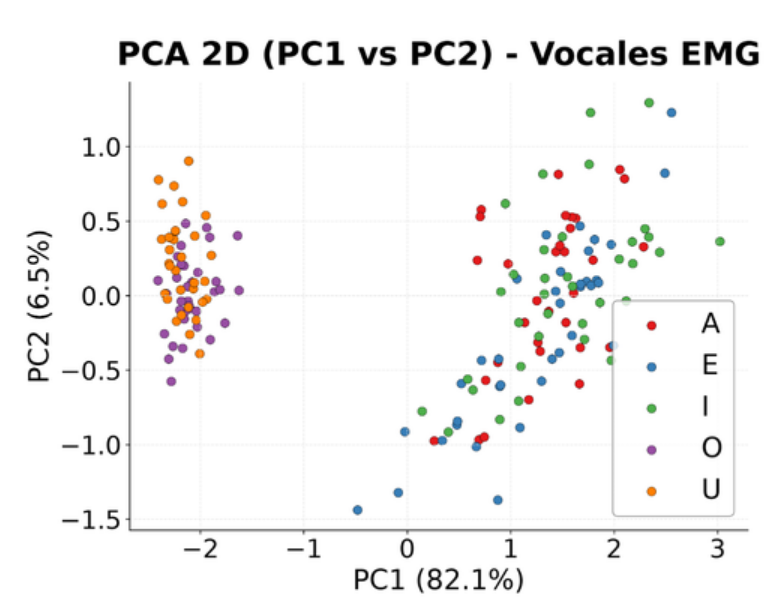
\includegraphics[width=\linewidth,height=0.29\textheight,keepaspectratio]{figuras/pca_vocales_modo_natural.png}\\[2pt]
            {\scriptsize \textbf{Modo Gesto Forzado: Separación Neta de I}}\\[1pt]
            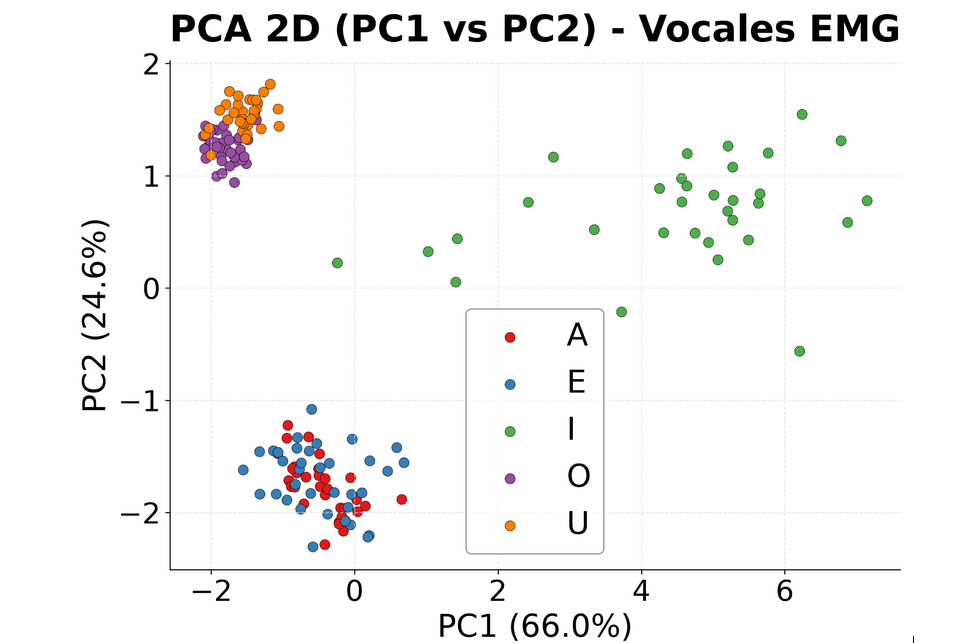
\includegraphics[width=\linewidth,height=0.29\textheight,keepaspectratio]{figuras/pca_vocales_modo_forzado.png}
        \end{column}
    \end{columns}
\end{frame}
